%\documentclass{article}
\documentclass[10pt,a4paper]{article}
\usepackage[a4paper,bindingoffset=0.2in,%
            left=1in,right=1in,top=1in,bottom=1in,%
            footskip=.25in]{geometry}



\usepackage[utf8]{inputenc}

\title{Solutions - Christian Thierfelder}
%\autor{}
%\date{}


%MATH
\usepackage{amsmath}
\usepackage{amsfonts}
\usepackage{amsthm}
\usepackage{amsbsy}
\usepackage{cancel}

\usepackage{algorithm}
\usepackage{algorithmic}

\usepackage{units}
\usepackage{mathrsfs}
\usepackage{slashed}
\usepackage{mathtools} %\mathclap - underbrace

\usepackage{hyperref}


\newtheorem{remark}{Remark}[section]
\theoremstyle{definition}
\newtheorem{definition}{Definition}[section]
\newtheorem{theorem}{Theorem}[section]

\DeclareMathOperator{\Aut}{Aut}
\DeclareMathOperator{\GL}{GL}

%PAGELAYOUT
\usepackage{a4wide}

%GRAPHICS
\usepackage{graphicx}
\usepackage[dvipsnames]{xcolor}
\usepackage{tikz}
\usepackage[outline]{contour} % glow around text
\usepackage{xfrac}

\usetikzlibrary{shapes}
\usetikzlibrary{plotmarks}
\usetikzlibrary{decorations.markings}

\usepackage{pgfplots}
\usepgfplotslibrary{polar}

%HYPERLINKS
\usepackage{hyperref}
\hypersetup{
    colorlinks=true,
    linkcolor=blue,
    filecolor=magenta,      
    urlcolor=cyan,
}

\usepackage[shortlabels]{enumitem}

\usepackage{etoolbox}
\providetoggle{includeCoverPic}
\settoggle{includeCoverPic}{true}
%\settoggle{includeCoverPic}{false}
\usepackage{subfiles}

\tikzset{>=latex} % for LaTeX arrow head
\colorlet{myred}{red!85!black}
\colorlet{mydarkred}{red!55!black}
\colorlet{mylightred}{red!85!black!12}
\colorlet{myfieldred}{mydarkred!5} % for S' background
\colorlet{myredhighlight}{myred!20} % highlights simultaneity in ladder paradox
\colorlet{myblue}{blue!80!black}
\colorlet{mydarkblue}{blue!50!black}
\colorlet{mylightblue}{blue!50!black!30}
\colorlet{mylightblue2}{myblue!10}
\colorlet{mygreen}{green!80!black}
\colorlet{mypurple}{blue!40!red!80!black}
\colorlet{mydarkgreen}{green!50!black}
\colorlet{mydarkpurple}{blue!40!red!50!black}
\colorlet{myorange}{orange!40!yellow!95!black}
\colorlet{mydarkorange}{orange!40!yellow!85!black}
\colorlet{mybrown}{brown!20!orange!90!black}
\colorlet{mydarkbrown}{brown!20!orange!55!black}
\colorlet{mypurplehighlight}{mydarkpurple!20} % highlights simultaneity in ladder paradox
\tikzstyle{world line}=[myblue!40,line width=0.3]
\tikzstyle{world line t}=[mypurple!50!myblue!40,line width=0.3]
\tikzstyle{world line'}=[mydarkred!40,line width=0.3]
\tikzstyle{mysmallarr}=[-{Latex[length=3,width=2]},thin]
\tikzstyle{mydashed}=[dash pattern=on 3 off 3]
\def\Nsamples{100}
\tikzstyle{vector}=[->,line width=1,line cap=round]
\tikzstyle{vector'}=[vector,shorten >=1.2]
\tikzstyle{particle}=[mygreen,line width=0.9]

\begin{document}

\maketitle
\section*{Advanced Topics in Gravity – Exercise sheet 6 - 2025-07-09}
\subsection*{Exercise 1 - Klein-Gordon inner product}
{\color{blue}

Prove, by considering two different Cauchy surfaces $\Sigma_1$ and $\Sigma_2$, that the Klein-Gordon inner product
\begin{equation}
(\phi_1, \phi_2) = -i \int_{\Sigma} d^3x \, \sqrt{h} \, n^{\mu} \bigl( \phi_1 D_{\mu} \phi_2^* - \phi_2^* D_{\mu} \phi_1 \bigr)
\end{equation}
is independent of the choice of the Cauchy surface.
}

With KG in curved space
\begin{align}
(D_\mu D^\mu+m^2)\phi=0
\end{align}
Observation (in analogy to 2nd order ODE's define a Wronskian)
\begin{align}
W_\mu&\equiv(D_\mu\phi_1)\phi_2^*-\phi_1(D_\mu\phi_2^*)\\
D^\mu W_\mu
&=(D^\mu D_\mu\phi_1)\phi_2^*+\cancel{(D_\mu\phi_1)(D^\mu\phi_2^*)}-\cancel{(D^\mu\phi_1)(D_\mu\phi_2^*)}-\phi_1(D^\mu D_\mu\phi_2^*)\\
&=(D^\mu D_\mu\phi_1)\phi_2^*-\phi_1(D^\mu D_\mu\phi_2^*)\\
&=-m^2\phi_1\phi_2^*-\phi_1(-m^2\phi_2^*)\\
&=0
\end{align}
With the covariant divergence theorem
\begin{align}
\int_{\partial\Omega} T^\mu\sqrt{-g}dS_\mu=\int_\Omega D_\mu T^\mu\sqrt{-g}d\Omega
\end{align}
we define a 4-volume $\Omega$ between the two Cauchy Surfaces $\Sigma_{1,2}$ and use $T=W$.  Then the (taking into account the orientation of top and bottom)
\begin{align}
0&=
\int_\Omega \underbrace{D_\mu W^\mu}_{=0}\sqrt{-g}d\Omega
=\int_{\partial\Omega} W^\mu\sqrt{-g}dS_\mu\\
&=
\int_{\Sigma_1} d^3x \, \sqrt{h} \, n^{\mu} \bigl( \phi_1 D_{\mu} \phi_2^* - \phi_2^* D_{\mu} \phi_1 \bigr)+\int_{\Sigma_2} d^3x \, \sqrt{h} \, (-n^{\mu}) \bigl( \phi_1 D_{\mu} \phi_2^* - \phi_2^* D_{\mu} \phi_1 \bigr)
\end{align}
resulting in
\begin{align}
\int_{\Sigma_1} d^3x \, \sqrt{h} \, n^{\mu} \bigl( \phi_1 D_{\mu} \phi_2^* - \phi_2^* D_{\mu} \phi_1 \bigr)=\int_{\Sigma_2} d^3x \, \sqrt{h} \, n^{\mu} \bigl( \phi_1 D_{\mu} \phi_2^* - \phi_2^* D_{\mu} \phi_1 \bigr)
\end{align}

\subsection*{Exercise 2 - Bogoliubov transformation}
{\color{blue}
We have seen that any field solution to the Klein-Gordon equation of motion can be expanded in terms of two bases:
\begin{equation}
\varphi = \sum_i \bigl( a_i f_i + a_i^\dagger f_i^* \bigr) = \sum_i \bigl( b_i g_i + b_i^\dagger g_i^* \bigr), 
\tag{2.1}
\end{equation}
where the basis modes are defined in different stationary regions and are normalized with respect to the Klein-Gordon inner product.  

Thus, the operators in the expansions satisfy
\begin{equation}
[ a_k, a_{k'}^\dagger ] = \delta(k - k'), 
\qquad
[ b_p, b_{p'}^\dagger ] = \delta(p - p').
\tag{2.2}
\end{equation}
The modes in the basis $\{g_i, g_i^*\}$ can be expressed in terms of the basis $\{f_j, f_j^*\}$ as
\begin{align}
g_i &= \sum_j \bigl( A_{ij} f_j + B_{ij} f_j^* \bigr), 
\tag{2.3}
\\
g_i^* &= \sum_j \bigl( B^*_{ij} f_j + A^*_{ij} f_j^* \bigr).
\tag{2.4}
\end{align}
This relation between the two bases is called a \emph{Bogoliubov transformation}, and it can also be written in matrix form as
\begin{equation}
\begin{pmatrix}
g \\
g^*
\end{pmatrix}
=
\begin{pmatrix}
A & B \\
B^* & A^*
\end{pmatrix}
\begin{pmatrix}
f \\
f^*
\end{pmatrix}.
\tag{2.5}
\end{equation}
\textit{Note}: The basis is normalized in such a way that
\[
(\alpha f, \beta g) = \alpha \beta^* (f, g),
\]
where $\alpha, \beta$ are any Bogoliubov coefficients and $f,g$ are any set of modes from the bases.

\begin{enumerate}
\item From the condition $(g_i, g_j) = \delta_{ij}$, find the relation:
\begin{equation}
A A^\dagger - B B^\dagger = 1.  \tag{2.6}
\end{equation}
    
\item From the condition $(g_i, g_j^*) = 0$, find the relation:
\begin{equation}
A B^{\mathrm{t}} - B A^{\mathrm{t}} = 0.  \tag{2.7}
\end{equation}

   
\item See how the previous relations (2.6) and (2.7) allow us to write the inverse matrix for the transformation.

\item By writing the field expansion in a matrix form as
\begin{equation}
\varphi = 
        \begin{pmatrix}
            b & b^\dagger
        \end{pmatrix}
        \begin{pmatrix}
            g \\ g^*
        \end{pmatrix}
        = 
        \begin{pmatrix}
            a & a^\dagger
        \end{pmatrix}
        \begin{pmatrix}
            f \\ f^*
        \end{pmatrix},
        \tag{2.8}
\end{equation}
and using the Bogoliubov transformations, write in a matrix form the relation between creation/annihilation operators with respect to the two different bases, i.e., find $M'$ such that
\begin{equation}
\begin{pmatrix}
   b \\ b^\dagger
\end{pmatrix}
= 
M'
\begin{pmatrix}
   a \\ a^\dagger
\end{pmatrix}. \tag{2.9}
\end{equation}
    
\end{enumerate}

}

\begin{enumerate}
\item
\begin{align}
(g_i,g_j)
&= \left(\sum_k ( A_{ik} f_k + B_{ik} f_k^*),\sum_l ( A_{jl} f_l + B_{jl} f_l^*)\right)\\
&= \sum_{k,l}\left( A_{ik} f_k + B_{ik} f_k^*, A_{jl} f_l + B_{jl} f_l^*\right)\\
&= \sum_{k,l}A_{ik}A^*_{jl}\underbrace{(f_k,f_l)}_{=\delta_{kl}}
+\sum_{k,l}A_{ik}B^*_{jl}\underbrace{(f_k,f_l^*)}_{=0}
+\sum_{k,l}B_{ik}A^*_{jl}\underbrace{(f_k^*,f_l)}_{=0}
+\sum_{k,l}B_{ik}B^*_{jl}\underbrace{(f_k^*,f_l^*)}_{=-\delta_{kl}}\\
&= \sum_{k}A_{ik}A^*_{jk}-B_{ik}B^*_{jk}\\
&\overset{!}{=}\delta_{ij}\quad\rightarrow AA^\dagger-BB^\dagger=1
\end{align}

\item
\begin{align}
(g_i,g^*_j)
&= \left(\sum_k ( A_{ik} f_k + B_{ik} f_k^*),\sum_l ( A_{jl} f_l + B_{jl} f_l^*)^*\right)\\
&= \sum_{k,l}\left( A_{ik} f_k + B_{ik} f_k^*, A^*_{jl} f^*_l + B^*_{jl} f_l\right)\\
&= \sum_{k,l}A_{ik}A_{jl}\underbrace{(f_k,f^*_l)}_{=0}
+\sum_{k,l}A_{ik}B_{jl}\underbrace{(f_k,f_l)}_{=\delta_{kl}}
+\sum_{k,l}B_{ik}A_{jl}\underbrace{(f_k^*,f_l^*)}_{=-\delta_{kl}}
+\sum_{k,l}B_{ik}B_{jl}\underbrace{(f_k^*,f_l)}_{=0}\\
&= \sum_{k}A_{ik}B_{jk}-B_{ik}A_{jk}\\
&=0\quad\rightarrow AB^t-BA^t=0
\end{align}

\item We use the proved equations above and extend them by 
\begin{align}
AA^\dagger-BB^\dagger=1\quad\rightarrow\quad A^*A^t-B^*B^t=1\\
AB^t-BA^t=0\quad\rightarrow\quad A^*B^\dagger-B^*A^\dagger=0
\end{align}
using $A^\dagger\equiv(A^*)^t\equiv(A^t)^*$. Using the four identities we can guess the inverse
\begin{align}
M^{-1}=
\left(\begin{matrix}
A^\dagger & -B^t\\
-B^\dagger & A^t
\end{matrix}\right).
\end{align}
Checking the result
\begin{align}
\left(\begin{matrix}
A &B\\
B^*&A^*
\end{matrix}\right)
\left(\begin{matrix}
A^\dagger & -B^t\\
-B^\dagger & A^t
\end{matrix}\right)
&=
\left(\begin{matrix}
AA^\dagger-BB^\dagger & -AB^t+BA^t\\
B^*A^\dagger-A^*B^\dagger & -B^*B^t+A^*A^t
\end{matrix}\right)
=
\left(\begin{matrix}
1 & 0\\
0 & 1
\end{matrix}\right).
\end{align}

\item With $\vec{a}^T\vec{f}=\phi=\vec{b}^T\vec{g}$ we see
\begin{align}
\vec{a}^T\vec{f}
=\phi
=\vec{b}^T\vec{g}
=(M'\vec{a})^T\vec{g}
=\vec{a}^TM'^T\vec{g}
=\vec{a}^TM'^TM\vec{f}
\end{align}
meaning $M'^TM=1\rightarrow M'^T=M^{-1}$ so
\begin{align}
M'=(M^{-1})^T=
\left(\begin{matrix}
A^\dagger & -B^\dagger\\
-B^t & A^t
\end{matrix}\right).
\end{align}


\end{enumerate}

\newpage
\section*{Advanced Topics in Gravity – Exercise sheet 5 - 2025-06-24}
\subsection*{Exercise 1 - Energy Conditions}
{\color{blue}

Analyze the different energy conditions: whether they hold, are violated, and which conditions must be satisfied if needed.

\begin{enumerate}
\item Consider a cosmological constant such that:
\begin{equation}
T^{(\Lambda)}_{\alpha\beta} = -\rho_\Lambda g_{\alpha\beta} \tag{1.1}
\end{equation}

where
\begin{align*}
\rho_\Lambda=-p_\Lambda = \frac{\Lambda}{8\pi G}, \quad \text{and} \quad \left(T_{\alpha\beta} - \frac{1}{2}g_{\alpha\beta}T\right) = \rho_\Lambda g_{\alpha\beta}.
\end{align*}


\item Consider a perfect fluid
\begin{equation}
T_{\alpha\beta} = (\rho + p)u_\alpha u_\beta + p g_{\alpha\beta}, \quad \text{with},\tag{1.2}
\end{equation}
with $g^{\alpha\beta} u_\alpha u_\beta = -1$ and
\begin{align*}
T^{\alpha}_{\ \alpha} = -\rho + 3p, \quad \text{so} \quad \left(T_{\alpha\beta} - \frac{1}{2}g_{\alpha\beta}T\right) = p_\Lambda g_{\alpha\beta}
\end{align*}


\subsubsection*{Note:}

These two exercises may be substituted for one of the analysis topics mentioned during the lecture today, such as:

\begin{itemize}
  \item Misner spacetime geodesics and lightcones
  \item Exotic matter and safety requirements for travellers in Morris-Thorne wormholes
\end{itemize}
\end{enumerate}
}

Taking the trace of the Einstein field equations (signature $[-,+,+,+]$)
\begin{align}
R_{\mu\nu}-\frac{1}{2}Rg_{\mu\nu}&=\kappa T_{\mu\nu}\\
\rightarrow R-\frac{1}{2}4R&=\kappa T\\
\rightarrow -R&=\kappa T\\
R_{\mu\nu}&=\kappa\left(T_{\mu\nu}-\frac{1}{2}Tg_{\mu\nu}\right)
\end{align}
where we used $g_{\mu\nu}g^{\nu\rho}=\delta^\rho_\mu$ and $g_{\mu\nu}g^{\mu\nu}=\delta^\mu_\mu=4$.

\begin{enumerate}
\item With EFE:
\begin{align}
R_{\mu\nu}-\frac{1}{2}Rg_{\mu\nu}&=\kappa\left(\underbrace{T_{\mu\nu}}_{\equiv0}-\frac{\Lambda}{\kappa} g_{\mu\nu}\right)\\
&=\kappa\underbrace{\left(-\frac{\Lambda}{\kappa} g_{\mu\nu}\right)}_{=T^\Lambda}
\end{align}
So we see that the cosmological constant can be understood as a special fluid with $p=-\Lambda/\kappa$ and $\rho=-p=\Lambda/\kappa$ 

\begin{itemize}
\item {\it WEC - weak energy condition $T_{\alpha\beta}t^\alpha t^\beta\ge0$ for all timelike $t^\alpha$ ($g_{\alpha\beta}t^\alpha t^\beta<0$)}
\begin{align}
T^\Lambda_{\alpha\beta}t^\alpha t^\beta
&=-\frac{\Lambda}{\kappa}\underbrace{g_{\alpha\beta}t^\alpha t^\beta}_{<0}\\
&=\frac{\Lambda}{\kappa}
\end{align}
Holds if $\Lambda\ge0$.
\item {\it NEC - null energy condition $T_{\alpha\beta}l^\alpha l^\beta\ge0$ for all null $l^\alpha$}
\begin{align}
T^\Lambda_{\alpha\beta}l^\alpha l^\beta
&=-\frac{\Lambda}{\kappa}\underbrace{g_{\alpha\beta}l^\alpha l^\beta}_{=0}\\
&=0
\end{align}
Holds.
\item {\it SEC - strong energy condition $(T_{\alpha\beta}-\frac{1}{2}Tg_{\alpha\beta})u^\alpha u^\beta\ge0$ for all unit timelike $u^\alpha$}
\begin{align}
(T^\Lambda_{\alpha\beta}-\frac{1}{2}T^\Lambda g_{\alpha\beta})u^\alpha u^\beta
&=\left[-\frac{\Lambda}{\kappa}-\frac{1}{2}4(-\frac{\Lambda}{\kappa}) \right]g_{\alpha\beta}u^\alpha u^\beta\\
&=-\frac{\Lambda}{\kappa}(-1)g_{\alpha\beta}u^\alpha u^\beta\\
&=\frac{\Lambda}{\kappa}g_{\alpha\beta}u^\alpha u^\beta\\
&=0
\end{align}
Holds if $\Lambda\ge0$

\item {\it DEC - Dominant energy condition $-T^\alpha_{\;\beta}u^\beta$ is a future directed timelike or null vector for all future directed timelike vectors $u^\alpha$}

For a perfect fluid the DEC holds when $\rho\ge|p|$. This means re require $\rho_\Lambda\ge|p_\Lambda|=\rho_\Lambda$ - so it holds.

\end{itemize}

\item {\bf The problem is a bit unclear - do we consider just a ideal fluid or fluid plus cosmological constant (there is a $p_\Lambda$ in the last equation)}.
We therefore consider the more complicated case and can set $\Lambda=0$ if needed

\begin{align}
R_{\mu\nu}-\frac{1}{2}Rg_{\mu\nu}
&=\kappa\left(T^\text{PF}_{\mu\nu}-\frac{\Lambda}{\kappa} g_{\mu\nu}\right)\\
&=\kappa\left((\rho+p)u_\mu u_\nu+pg_{\mu\nu}-\frac{\Lambda}{\kappa} g_{\mu\nu}\right)\\
&=\kappa\left((\rho+p)u_\mu u_\nu+\left[p-\frac{\Lambda}{\kappa}\right]g_{\mu\nu}\right)\\
\end{align}
then
\begin{align}
T_{\mu\nu}&=(\rho+p)u_\mu u_\nu+\left[p-\frac{\Lambda}{\kappa}\right]g_{\mu\nu}\\
\rightarrow T^\mu_{\;\mu}
&=(\rho+p)\underbrace{u^\mu u_\mu}_{=-1}+4\left[p-\frac{\Lambda}{\kappa}\right]\\
&=3p-\rho-4\frac{\Lambda}{\kappa}\\
\rightarrow T_{\mu\nu}-\frac{1}{2}g_{\mu\nu}T
&=(\rho+p)u_\mu u_\nu+\left[p-\frac{\Lambda}{\kappa}\right]g_{\mu\nu}-\frac{1}{2}(3p-\rho-4\frac{\Lambda}{\kappa})g_{\mu\nu}\\
&=(\rho+p)u_\mu u_\nu+\left[-\frac{1}{2}p+\frac{1}{2}\rho+\frac{\Lambda}{\kappa}\right]g_{\mu\nu}
\end{align}
\begin{itemize}
\item {\it WEC - weak energy condition $T_{\alpha\beta}t^\alpha t^\beta\ge0$ for all timelike $t^\alpha$ ($g_{\alpha\beta}t^\alpha t^\beta<0$)}
\begin{align}
T_{\alpha\beta}t^\alpha t^\beta
&=(\rho+p)\underbrace{u_\alpha u_\beta t^\alpha t^\beta}_{=(u_\alpha t^\alpha)^2\ge0}+\left[p-\frac{\Lambda}{\kappa}\right]\underbrace{g_{\alpha\beta}t^\alpha t^\beta}_{<0}
\end{align}
Holds if $p+\rho\ge0$ and $p-\frac{\Lambda}{\kappa}\ge0$.
\item {\it NEC - null energy condition $T_{\alpha\beta}l^\alpha l^\beta\ge0$ for all null $l^\alpha$}

See above - holds if $p+\rho\ge0$
\item {\it SEC - strong energy condition $(T_{\alpha\beta}-\frac{1}{2}Tg_{\alpha\beta})u^\alpha u^\beta\ge0$ for all unit timelike $u^\alpha$}
\begin{align}
(T_{\alpha\beta}-\frac{1}{2}T g_{\alpha\beta})u^\alpha u^\beta
&=(\rho+p)\underbrace{u_\alpha u_\beta u^\alpha u^\beta}_{=(u^2)^2=1}+\left[-\frac{1}{2}p+\frac{1}{2}\rho+\frac{\Lambda}{\kappa}\right]\underbrace{g_{\alpha\beta}u^\alpha u^\beta}_{=-1}\\
&=(\rho+p)+\left[\frac{1}{2}p-\frac{1}{2}\rho-\frac{\Lambda}{\kappa}\right]\\
&=\frac{1}{2}\left(3p+\rho+2\frac{\Lambda}{\kappa}\right)
\end{align}
Holds if $3p+\rho+2\frac{\Lambda}{\kappa}\ge0$

\item {\it DEC - Dominant energy condition $-T^\alpha_{\;\beta}u^\beta$ is a future directed timelike or null vector for all future directed timelike vectors $u^\alpha$}

For $\Lambda=0$ holds if $\rho\ge|p|$.
\end{itemize}

\item Safety requirements for travelers in Morris-Thorne wormholes

The general safety requirements (derived from what we know about Schwarzschild/Kerr BHs) are (independent of specific solution/shape of the wormhole)
\begin{itemize}
\item Small tidal forces - to avoid squeezing/streching
\item Small acceleration - to avoid trauma
\item No even horizon I - to avoid signal loss between brain and rest of the body - or weird quantum effects on atoms (nucleus inside EH - electrons outside)
\item No even horizon II - to be able to go back and forth (no sure if this counts as safety requirement)
\item Solution must be stable with respect to external perturbations - wormhole should not collapse when traveler passes through
\item Short transition time to other side - to avoid starvation/suffocation
\item Large enough passage - so whole body/ship fits through
\item Low radiation levels (Doppler shift of surrounding particles)
\end{itemize} 
I just found the paper - but haven't read it yet.


\end{enumerate}

\newpage
\section*{Advanced Topics in Gravity – Exercise sheet 4 - 2025-06-08}
\subsection*{Exercise 1 - Penrose diagrams}
{\color{blue} 
Depict the Penrose diagram of the Schwarzschild spacetime when it has negative mass. We recommend to follow these steps:
\begin{enumerate}
\item Write the negative-mass Schwarzschild metric and analyze it.
\item Write the coordinate transformation and give the conformally compactified metric.
\item Identify infinities and singularities.
\item Draw the diagram.
\end{enumerate}
Hint: Recall that this spacetime possesses a naked singularity. This kind of singularity is not covered by any horizon and it is going to be timelike.
}
\begin{enumerate}
\item With $\mu=-M>0$
\begin{align}
ds^2 = \left(1 + \frac{2G\mu}{r}\right) dt^2 - \left(1 + \frac{2G\mu}{r}\right)^{-1} dr^2 - r^2[d\vartheta^2+\sin^2\vartheta d\phi^2]
\end{align}
We see that the metric coefficient $g_{tt}>0$ everywhere - so there is no horizon. The center $r=0$ is still a singularity
\begin{align}
R^{\mu\nu\rho\sigma}R_{\mu\nu\rho\sigma}=\frac{48G^2\mu^2}{r^6}
\end{align}
but now it is naked (not covered by a horizon). The metric remains asymptotically flat for $r\rightarrow\infty$.
\item We define the tortoise coordinate again
\begin{align}
\frac{dr^*}{dr}&=\frac{1}{1+\frac{2G\mu}{r}}\\
\rightarrow r^*&=r-2G\mu\log\left[1+\frac{r}{2G\mu}\right]
\end{align}
And now we define advanced and retarded null-coordinates
\begin{align}
v&=t+r^*\qquad\\
u&=t-r^*\qquad
\end{align}
then
\begin{align}
\left(1+\frac{2G\mu}{r}\right)du dv 
&= \left(1+\frac{2G\mu}{r}\right)(dt-dr^*)(dt+dr^*)\\
&= \left(1+\frac{2G\mu}{r}\right)(dt^2-(dr^*)^2)\\
&=\left(1+\frac{2G\mu}{r}\right)dt^2-\frac{1}{1+\frac{2G\mu}{r}}dr^2
\end{align}
resulting in
\begin{align}
ds^2 = \left(1 + \frac{2G\mu}{r}\right) du\,dv - r^2[d\vartheta^2+\sin^2\vartheta d\phi^2]
\end{align}
Now we compactify ($\Omega=\cos U\cos V$)
\begin{align}
u&=\tan U\\
v&=\tan V\\
\rightarrow du\,dv&=\frac{1}{\cos^2U}\frac{1}{\cos^2V} dU\,dV\\
\rightarrow ds^2 &= \frac{1}{\cos^2U\,\cos^2V}\left(1 + \frac{2G\mu}{r}\right) dU\,dV - r^2[d\vartheta^2+\sin^2\vartheta d\phi^2]\\
&=\Omega^{-2}\left[\left(1 + \frac{2G\mu}{r}\right)dU\,dV - r^2\Omega^2(d\vartheta^2+\sin^2\vartheta d\phi^2)\right]
\end{align}
The boundary $\Omega=0$ is where $U=\pm\pi/2$ or $V=\pm\pi/2$ (or both), i.e.
$u,v=\pm\infty$. Since $r\Omega\neq 0$ (I checked with Mathematica) at $\Omega= 0$, the boundary consists of (pieces of) a light cone.
Now we do just a rotation to bring it into the normal shape of a Penrose diagram
\begin{align}
T&=\frac{1}{2}(V+U)\\
&=\frac{1}{2}(\arctan{v}+\arctan{u})\\
&=\frac{1}{2}(\arctan{[t+r^*]}+\arctan{[t-r^*]})\\
R&=\frac{1}{2}(V-U)\\
&=\frac{1}{2}(\arctan{v}-\arctan{u})\\
&=\frac{1}{2}(\arctan{[t+r^*]}-\arctan{[t-r^*]})
\end{align}
Then
\begin{align}
dU&=dT-dR,\qquad dV=dT+dR\\
\rightarrow dU dV&=dT^2-dR^2\\
ds^2&=\Omega^{-2}\left[\left(1 + \frac{2G\mu}{r}\right)(dT^2-dR^2) - r^2\Omega^2(d\vartheta^2+\sin^2\vartheta d\phi^2)\right]
\end{align}
So the spacetime is similar to a Minkowski space BUT with a singularity at $r=0$ 
\item See Mathematica code
\begin{itemize}
\item $r=0$ is the naked singularity
\item the null surface $V=\frac{1}{2}\pi$ called $\mathcal{I}^+$ (future lightlike infinity)
\item the null surface $U=-\frac{1}{2}\pi$ called $\mathcal{I}^-$ (past lightlike infinity)
\item the point $U=V=\pi/2$ is called $i^+$ (future timelike infinity)
\item the point $V=\pi/2, U=-\pi/2$ is called $i^0$ (spacelike infinity)
\end{itemize}
\item See Mathematica code ($r,t= $const. plotted for $\mu=1$)
\begin{figure}[!h]
\centering
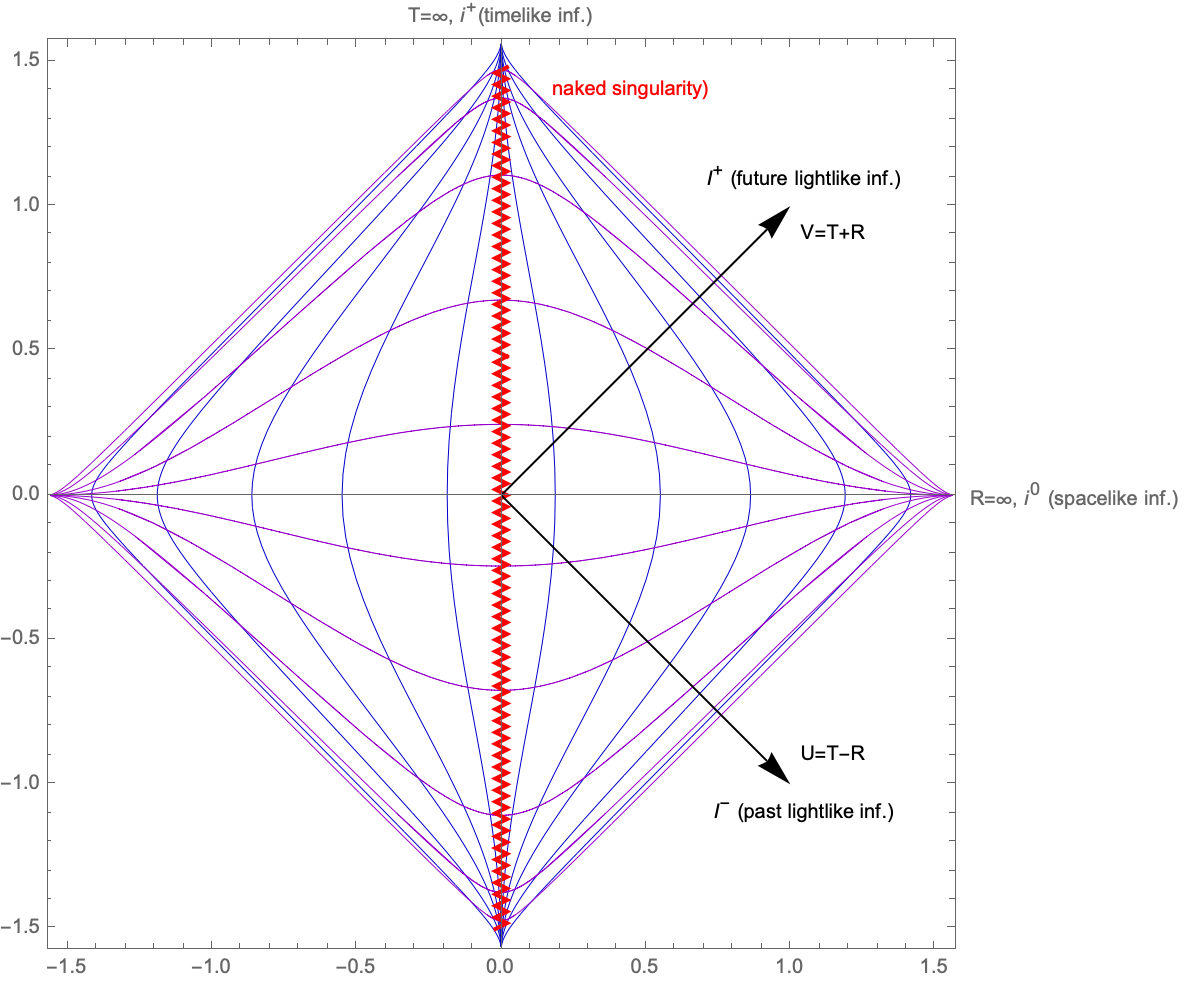
\includegraphics[width=0.9\textwidth]{/Users/christiant/MyDocuments/TeX/Hohm_AdvGR/pic_sheet4_1.png}
\caption{Mathematica calculations}
\end{figure}
\end{enumerate}

\newpage

\section*{Advanced Topics in Gravity – Exercise sheet 3 - 2025-05-27}
\subsection*{Exercise 1 - Killing vectors in Kerr spacetime}
{\color{blue}

\begin{enumerate}[1.)]
\item Check that Kerr spacetime has two Killing vector fields that can be expressed as
\begin{align}
\xi = \partial_t \quad \text{and} \quad \psi = \partial_\varphi.
\end{align}

\item Show that the hypersurfaces defined by $r = r_\pm$ are Killing horizons of the Killing vectors
\begin{align}
\chi_\pm = \xi + \Omega_H \psi,
\end{align}
where $\Omega_H = \frac{a}{2mr_\pm}$ is the angular velocity.

\item Show that the Killing vector $\chi_+ = \xi + \Omega_{H+} \psi$ is spacelike in the ergosphere region $r_+ < r < r_{E+}$.

\end{enumerate}
\bigskip
\noindent\textit{Note:} A Killing horizon is a null hypersurface endowed with a normal Killing vector, which is null at the hypersurface.
}

\begin{enumerate}
\item First lets make some general statement about Killing vectors: 

Let $x^\mu$ be a coordinate chart on a spacetime manifold \( \mathcal{M} \). A general Killing vector field $\xi$ needs to satisfy the Killing equation:
\begin{align}
(\mathcal{L}_\xi g)_{\mu\nu} = \xi^\sigma \partial_\sigma g_{\mu\nu} + g_{\sigma\nu} \partial_\mu \xi^\sigma + g_{\mu\sigma} \partial_\nu \xi^\sigma=0
\end{align}
where $\mathcal{L}_\xi$ denotes the Lie derivative with respect to $\xi$. In case of a  coordinate vector $\xi = \partial_\lambda$, we have $\xi^\sigma = \delta^\sigma_\lambda$, and thus:
\begin{align}
\partial_\mu \xi^\sigma = \partial_\nu \xi^\sigma = 0.
\end{align}
Therefore,
\begin{align}
(\mathcal{L}_\xi g)_{\mu\nu} = \partial_\lambda g_{\mu\nu}.
\end{align}
So we conclude: if a coordinate $x^\lambda$ do not appear in the metric components, the associated coordinate vector field $\xi^\sigma = \delta^\sigma_\lambda$ is a Killing vector field.

The Kerr solution in the Boyer–Lindquist (I might use a different signature the the lecture ) form is given by:
\begin{align}
ds^2 &= -\left(1-\frac{2mr}{\rho^2}\right)dt^2+\frac{\rho^2}{\Delta}dr^2+\rho^2d\theta^2+\left(r^2+a^2+\frac{2mra^2\sin^2\theta}{\rho^2}\right)\sin^2\theta\,d\phi^2-\frac{4Mra\sin^2\theta}{\rho^2}\,dtd\phi\\
\rho^2 &= r^2 + a^2 \cos^2\theta\\
\Delta &= r^2 - 2mr + a^2.
\end{align}
Since the coordinates $t$ and $\phi$ do not appear in the Kerr metric, the coordinate vector fields $\xi=\partial_t$, and $\psi=\partial_\phi$ are Killing vector fields.


\item Assuming $a^2<m^2$.
\begin{enumerate}
\item Then the normal co-vector field is given by 
\begin{align}
n_\mu&=(0,1,0,0)\\
\rightarrow n^\nu
&=g^{\nu\mu}n_\mu\\
&=(0,g^{rr},0,0)\\
\rightarrow n^2&=n^\mu n_\mu=g^{rr}
\end{align}
This means the hypersurfaces $r = \text{constant}$ becomes null, 
when $g^{rr}$ (of the inverse metric) vanishes.

From the Boyer–Lindquist form, we find
\begin{align}
g^{rr}&=\frac{\Delta}{\rho^2}=\frac{r^2-2mr+a^2}{r^2+a^2\cos^\theta}\overset{!}{=}0\\
\rightarrow\Delta&=r^2-2mr+a^2=0\\
\rightarrow r_\pm&=m\pm\sqrt{m^2-a^2}
\end{align}

\item Now we are calculating with Mathematica
\begin{align}
g&_{\mu\nu}\chi^\mu\chi^\nu\\
&=\left(1,0,\frac{a}{2mr_\pm},0\right)g_{\mu\nu}|_{r=r_\pm}
\left(\begin{matrix}
1\\
0\\
\frac{a}{2mr_\pm}\\
0
\end{matrix}\right)\\
&=g_{tt}+2g_{t\phi}\frac{a}{2mr_\pm}+g_{\phi\phi}\frac{a^2}{4m^2r^2_\pm}\\
&=0
\end{align}
so the Killing vector is null at the hypersurface.
\begin{figure}[!h]
\centering
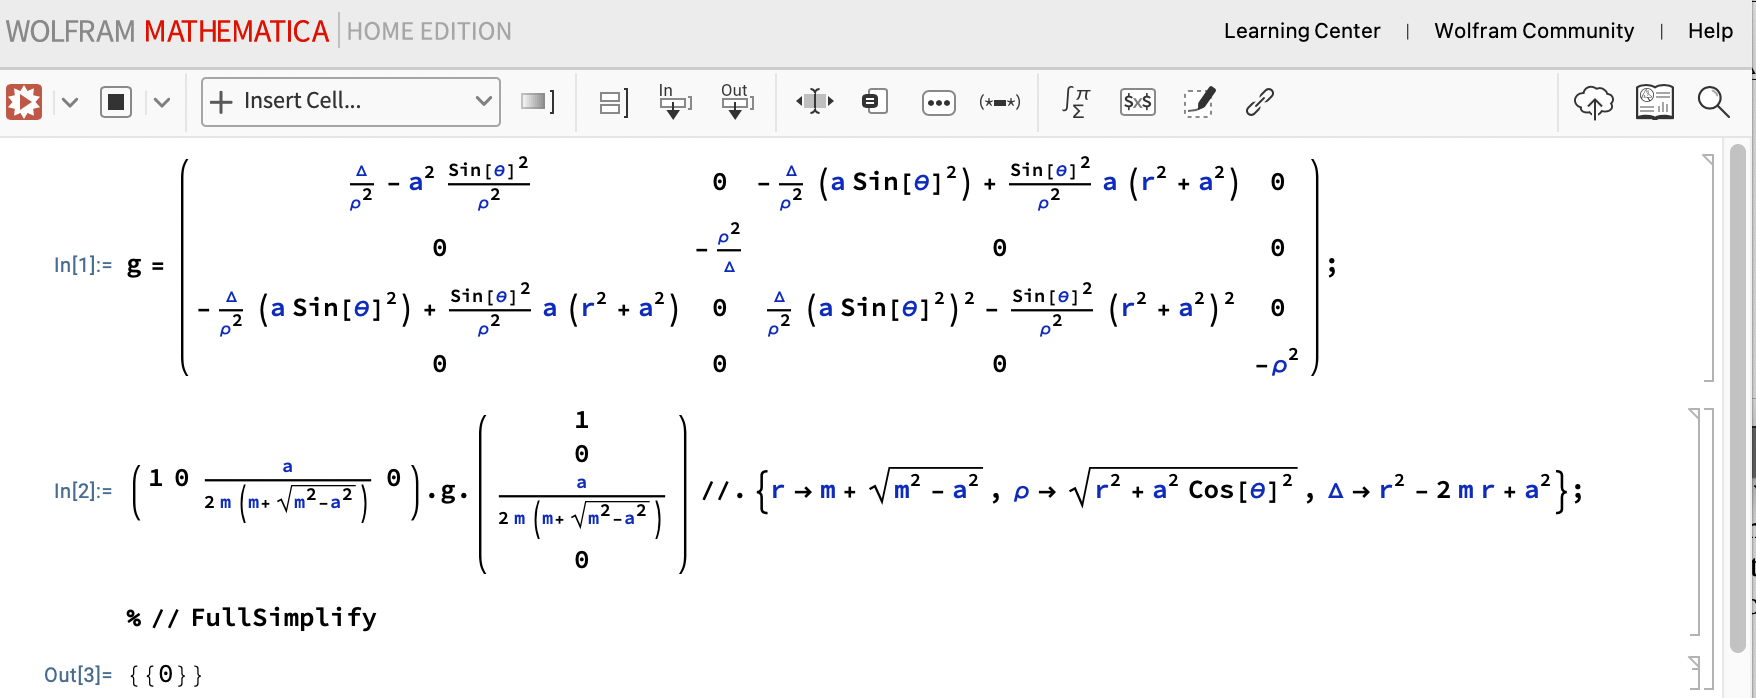
\includegraphics[width=0.9\textwidth]{/Users/christiant/MyDocuments/TeX/Hohm_AdvGR/pic_sheet3_1.png}
\caption{Mathematica calculations}
\end{figure}
\end{enumerate}

\item With 
\begin{align}
r_+&=m+\sqrt{m^2-a^2}\\
r_{E+}&=m+\sqrt{m^2-a^2\cos^2\theta}
\end{align}
For $\chi_+$ to be spacelike we calculate
\begin{align}
g_{\mu\nu}&\chi^\mu_+\chi^\nu_+
=g_{tt}\cdot 1+2\Omega_{H+}g_{t\phi}+\Omega_{H+}^2g_{\phi\phi}\\
&=\frac{1}{2} \left(\frac{a \sin ^2(\theta ) \left(\frac{2 a^2 m r \sin ^2(\theta )}{a^2 \cos ^2(\theta
   )+r^2}+a^2+r^2\right)}{m \left(\sqrt{m^2-a^2}+m\right)}+\frac{4 m r}{a^2 \cos ^2(\theta
   )+r^2}-\frac{a^3 r \sin ^2(\theta )}{m \left(\sqrt{m^2-a^2}+m\right)^2 \left(a^2 \cos ^2(\theta
   )+r^2\right)}-2\right)
\end{align}
This looks quite ugly - therefore lets check the components
\begin{itemize}
\item Checking the terms
\begin{align}
g_{tt}
&=-\frac{r^2+a^2\cos^2\theta-2mr}{r^2+a^2\cos^2\theta}\\
\rightarrow g_{tt}&\overset{!}{=}0\\
\rightarrow r&=m\pm\sqrt{m^2-a^2\cos^2\theta}=r_{E+}\\
g_{tt}(r_+)&>0
\end{align}
So $g_{tt}$ is positive is ergosphere and vanishes at $r_{E+}$. This implies $\xi=\partial_t$ is spacelike.
\item Next is $g_{\phi\phi}$. 
\begin{align}
g_{\phi\phi}
&=\left(r^2+a^2+\frac{2mra^2\sin^2\theta}{r^2 + a^2 \cos^2\theta}\right)\sin^2\theta\\
&>0
\end{align}
This implies $\psi=\partial_\phi$ is spacelike (because $\Omega_{H+}>0$).
\item And
\begin{align}
g_{t\phi}
&=-\frac{2mar\sin^2\theta}{r^2 + a^2 \cos^2\theta}\\
&<0
\end{align}
which makes the whole makes the analysis inconclusive.
\end{itemize}
But with the use of Mathematica I could show analytically that $g_{\mu\nu}\chi^\mu_+\chi^\nu$ is spacelike in the ergoshperes equatorial plane - so there might be some argument (which I do not have) to conclude that this holds in the whole ergoshpere.


\end{enumerate}

\newpage
\section*{Advanced Topics in Gravity – Exercise sheet 2 - 2025-05-14}
\subsection*{Exercise 1 - Extension of Schwarzschild metric}
{\color{blue}
\begin{enumerate}
\item Write the retarded null metric in terms of the retarded null coordinate $u = t- r^*$.
\item Draw the behaviour of light cones in the advanced null coordinates.
\item Show that $\dot{u} = 0$ and $\dot{v} = 0$ are radial null geodesics with a finite value at $r = 2GM$.
\end{enumerate}
}

\begin{enumerate}
\item The actual definition of tortoise coordinates is given by the ODE 
\begin{align}
\frac{dr^*}{dr}&=\frac{1}{1-\frac{2GM}{r}}\\
\rightarrow r^*&=\int \frac{1}{1-\frac{2GM}{r}}dr\\
&=r+2GM\log\left(r-2GM\right)+C\\
&=r+2GM\log\left(\frac{r}{2GM}-1\right).
\end{align}
With $u = t- r^*$ and $A\equiv1-\frac{2GM}{r}$
\begin{align}
\rightarrow dr^*&=dr+\frac{dr}{\frac{r}{2GM}-1}\\
&=\frac{dr}{1-\frac{2GM}{r}}=\frac{1}{A}dr\\
\rightarrow du&=dt-dr^*\\
&=dt-\frac{1}{A}dr
\end{align}
then
\begin{align}
du^2&=dt^2-2dt\,dr^*+(dr^*)^2\\
&=dt^2-\frac{2}{A}dt\,dr+\frac{1}{A^2}dr^2\\
du\,dr&=dt\,dr-\frac{1}{A}dr^2\\
\rightarrow A\,du^2+2du\,dr&=A\,dt^2-2dt\,dr+\frac{1}{A}dr^2+2dt\,dr-\frac{2}{A}dr^2\\
&=A\,dt^2-\frac{1}{A}dr^2
\end{align}
and substituding into the Schwarzschild metric
\begin{align}
ds^2
&=A\,dt^2-\frac{1}{A}dr^2-r^2d\Omega\\
&=A\,du^2+2du\,dr-r^2d\Omega\\
&=\left(1-\frac{2GM}{r}\right)du^2+2du\,dr-r^2d\Omega
\end{align}
\item Coordinate overview for $r>2M$
\begin{table}[!h]
\centering
\begin{tabular}{lccc}
\hline\hline
&& \multicolumn{2}{c}{radial null geodesic $(ds=0, d\Omega=0)$}\\
coordinates &  metric &  in &  out\\
\hline
Schwarzschild &	 $ds^2=A\,dt^2-\frac{1}{A}dr^2-r^2d\Omega$ & $\frac{dt}{dr}=+A$ & $\frac{dt}{dr}=-A$\\
\\
$t\rightarrow u=t-r^*$\\
retarded null coordinate   & $ds^2=A\,du^2+2du\,dr-r^2d\Omega$ & $\frac{du}{dr}=-2/A$ & $du=0$\\
(ret. Eddington-Finkelstein)\\
\\
$t\rightarrow v=t+r^*$\\
advanced null coordinate  & $ds^2=A\,dv^2-2dv\,dr-r^2d\Omega$ & $dv=0$ & $\frac{dv}{dr}=2/A$\\
(adv. Eddington-Finkelstein)\\
\hline\hline
\end{tabular}
\end{table}

In the $v-r$ diagram ($v=$const are horizontal lines) we see the light cones ({\bf angle between in and outgoing null geodesic}) laying on the left side 
\begin{figure}[!h]
\centering
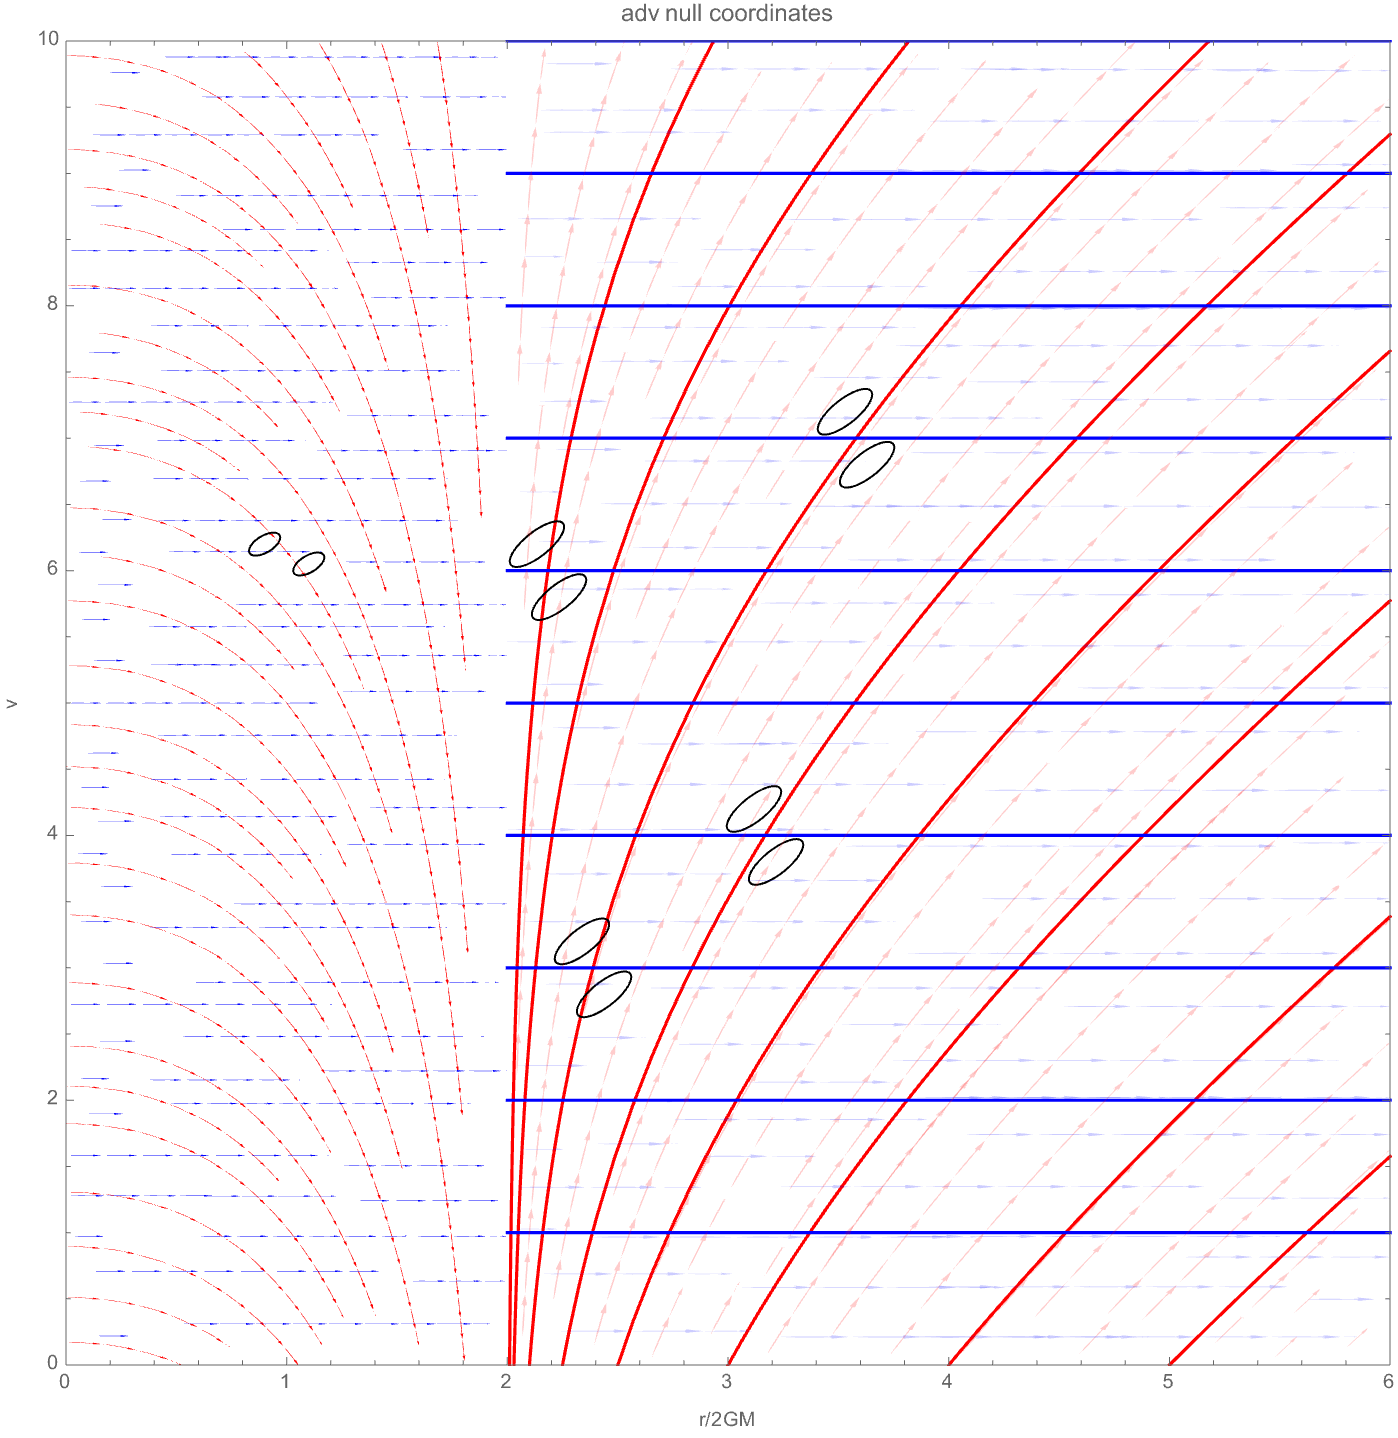
\includegraphics[width=0.7\textwidth]{/Users/christiant/MyDocuments/TeX/Hohm_AdvGR/pic_Sheet2_1.png}
\caption{Advanced null coordinate: $v-r$-diagram }
\end{figure}

\begin{figure}[!h]
\centering
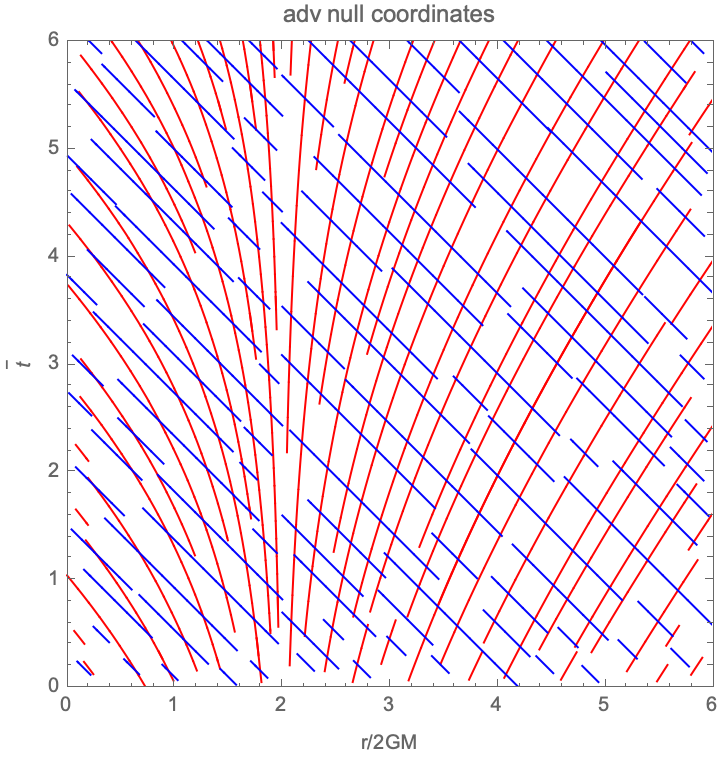
\includegraphics[width=0.7\textwidth]{/Users/christiant/MyDocuments/TeX/Hohm_AdvGR/pic_Sheet2_1b.png}
\caption{Advanced null coordinate: $\bar{t}-r$-diagram }
\end{figure}

Alternatively we could have plotted a $\bar{t}-r$ diagram where $v=$const are 45 degree diagonals.
\begin{align}
ds^2&=\left(1-\frac{2GM}{r}\right)d\bar{t}^2-\frac{4GM}{4}d\bar{t}dr-\left(1-\frac{2GM}{r}\right)dr^2-r^2d\Omega\\
\rightarrow& \left(1-\frac{2GM}{r}\right)\left(\frac{d\bar{t}}{dr}\right)^2-\frac{4G M}{r}\frac{d\bar{t}}{dr}=\left(1+\frac{2GM}{r}\right)\\
\rightarrow& \frac{d\bar{t}}{dr}=-\frac{2GM+\sqrt{8G^2M^2-4GMr+r^2}}{2GM-r}
\end{align}

\item Assumptions
\begin{itemize}
\item null geodesic: $ds=0$
\item radial: $\dot{\theta}=0=\dot{\phi}$
\end{itemize}
\begin{itemize}[(a)]
\item Retarded null coordinates: line element and geodesic equation
\begin{align}
g_{bc}\frac{dx^b}{d\lambda}\frac{dx^c}{d\lambda}&=0\\
\frac{d^2x^a}{d\lambda^2}+\Gamma^a_{bc}\frac{dx^b}{d\lambda}\frac{dx^c}{d\lambda}&=0
\end{align}
obtaining
\begin{align}
2\dot{r}\dot{u}+\left(1-\frac{2GM}{r^2}\right)\dot{u}^2-r^2\dot{\theta}^2-r^2\sin^2\theta\dot{\phi}^2&=0\\
\ddot{u}-\frac{GM}{r^2}\dot{u}^2+r\dot{\theta}^2+r\sin^2\theta\dot{\phi}^2&=0\\
\ddot{r}+\frac{2GM}{r^2}\dot{u}\dot{r}+(2GM-r)\dot{\theta}^2+\frac{GM(r-2GM)}{r^3}\dot{u}^2+(2GM-r)\sin^2\theta\dot{\phi}^2&=0\\
\ddot{\theta}+\frac{2}{r}\dot{r}\dot{\theta}-\sin\theta\cos\theta\;\dot{\phi}^2&=0\\
\ddot{\phi}+\frac{2}{r}\dot{r}\dot{\phi}+2\cot\theta\;\dot{\phi}\dot{\theta}&=0
\end{align}
Inserting $\dot{\phi}=0=\dot{\theta}$ (radial geodesic)
\begin{align}
2\dot{r}\dot{u}+\left(1-\frac{2GM}{r^2}\right)\dot{u}^2&=0\qquad\rightarrow\dot{u}=0\qquad\text{or }\dot{r}=1/(1-2GM/r)\\
\ddot{u}-\frac{GM}{r^2}\dot{u}^2&=0\\
\ddot{r}+\frac{2GM}{r^2}\dot{u}\dot{r}+\frac{GM(r-2GM)}{r^3}\dot{u}^2&=0
\end{align}
We see $\dot{u}=0$ with $\dot{\phi}=0, \dot{\theta}=0, r=c_1\lambda+c_2$ is null geodesic with a finite value at $r=2GM$.

\item Advanced null coordinates: line element and geodesic equation
\begin{align}
-2\dot{r}\dot{v}+\left(1-\frac{2GM}{r^2}\right)\dot{v}^2-r^2\dot{\theta}^2-r^2\sin^2\theta\dot{\phi}^2&=0\\
\ddot{v}+\frac{GM}{r^2}\dot{v}^2-r\dot{\theta}^2-r\sin^2\theta\dot{\phi}^2&=0\\
\ddot{r}-\frac{2GM}{r^2}\dot{v}\dot{r}+(2GM-r)\dot{\theta}^2+\frac{GM(r-2GM)}{r^3}\dot{v}^2+(2GM-r)\sin^2\theta\dot{\phi}^2&=0\\
\ddot{\theta}+\frac{2}{r}\dot{r}\dot{\theta}-\sin\theta\cos\theta\;\dot{\phi}^2&=0\\
\ddot{\phi}+\frac{2}{r}\dot{r}\dot{\phi}+2\cot\theta\;\dot{\phi}\dot{\theta}&=0
\end{align}
Inserting $\dot{\phi}=0=\dot{\theta}$ (radial geodesic)
\begin{align}
-2\dot{r}\dot{v}+\left(1-\frac{2GM}{r^2}\right)\dot{v}^2&=0\qquad\rightarrow\qquad\dot{v}=0\\
\ddot{v}+\frac{GM}{r^2}\dot{v}^2&=0\\
\ddot{r}-\frac{2GM}{r^2}\dot{v}\dot{r}+\frac{GM(r-2GM)}{r^3}\dot{v}^2&=0
\end{align}
We see again $\dot{v}=0$ with $\dot{\phi}=0, \dot{\theta}=0, r=c_1\lambda+c_2$ is null geodesic with a finite value at $r=2GM$.

\end{itemize}
\end{enumerate}

\newpage
\section*{Advanced Topics in Gravity – Exercise sheet 1 - 2025-04-29}
\subsection*{Exercise 1 - Friedmann-Robertson-Walker metric}

\begin{enumerate}[1.]
\item Mathematica calculation gives
\begin{figure}[!h]
\centering
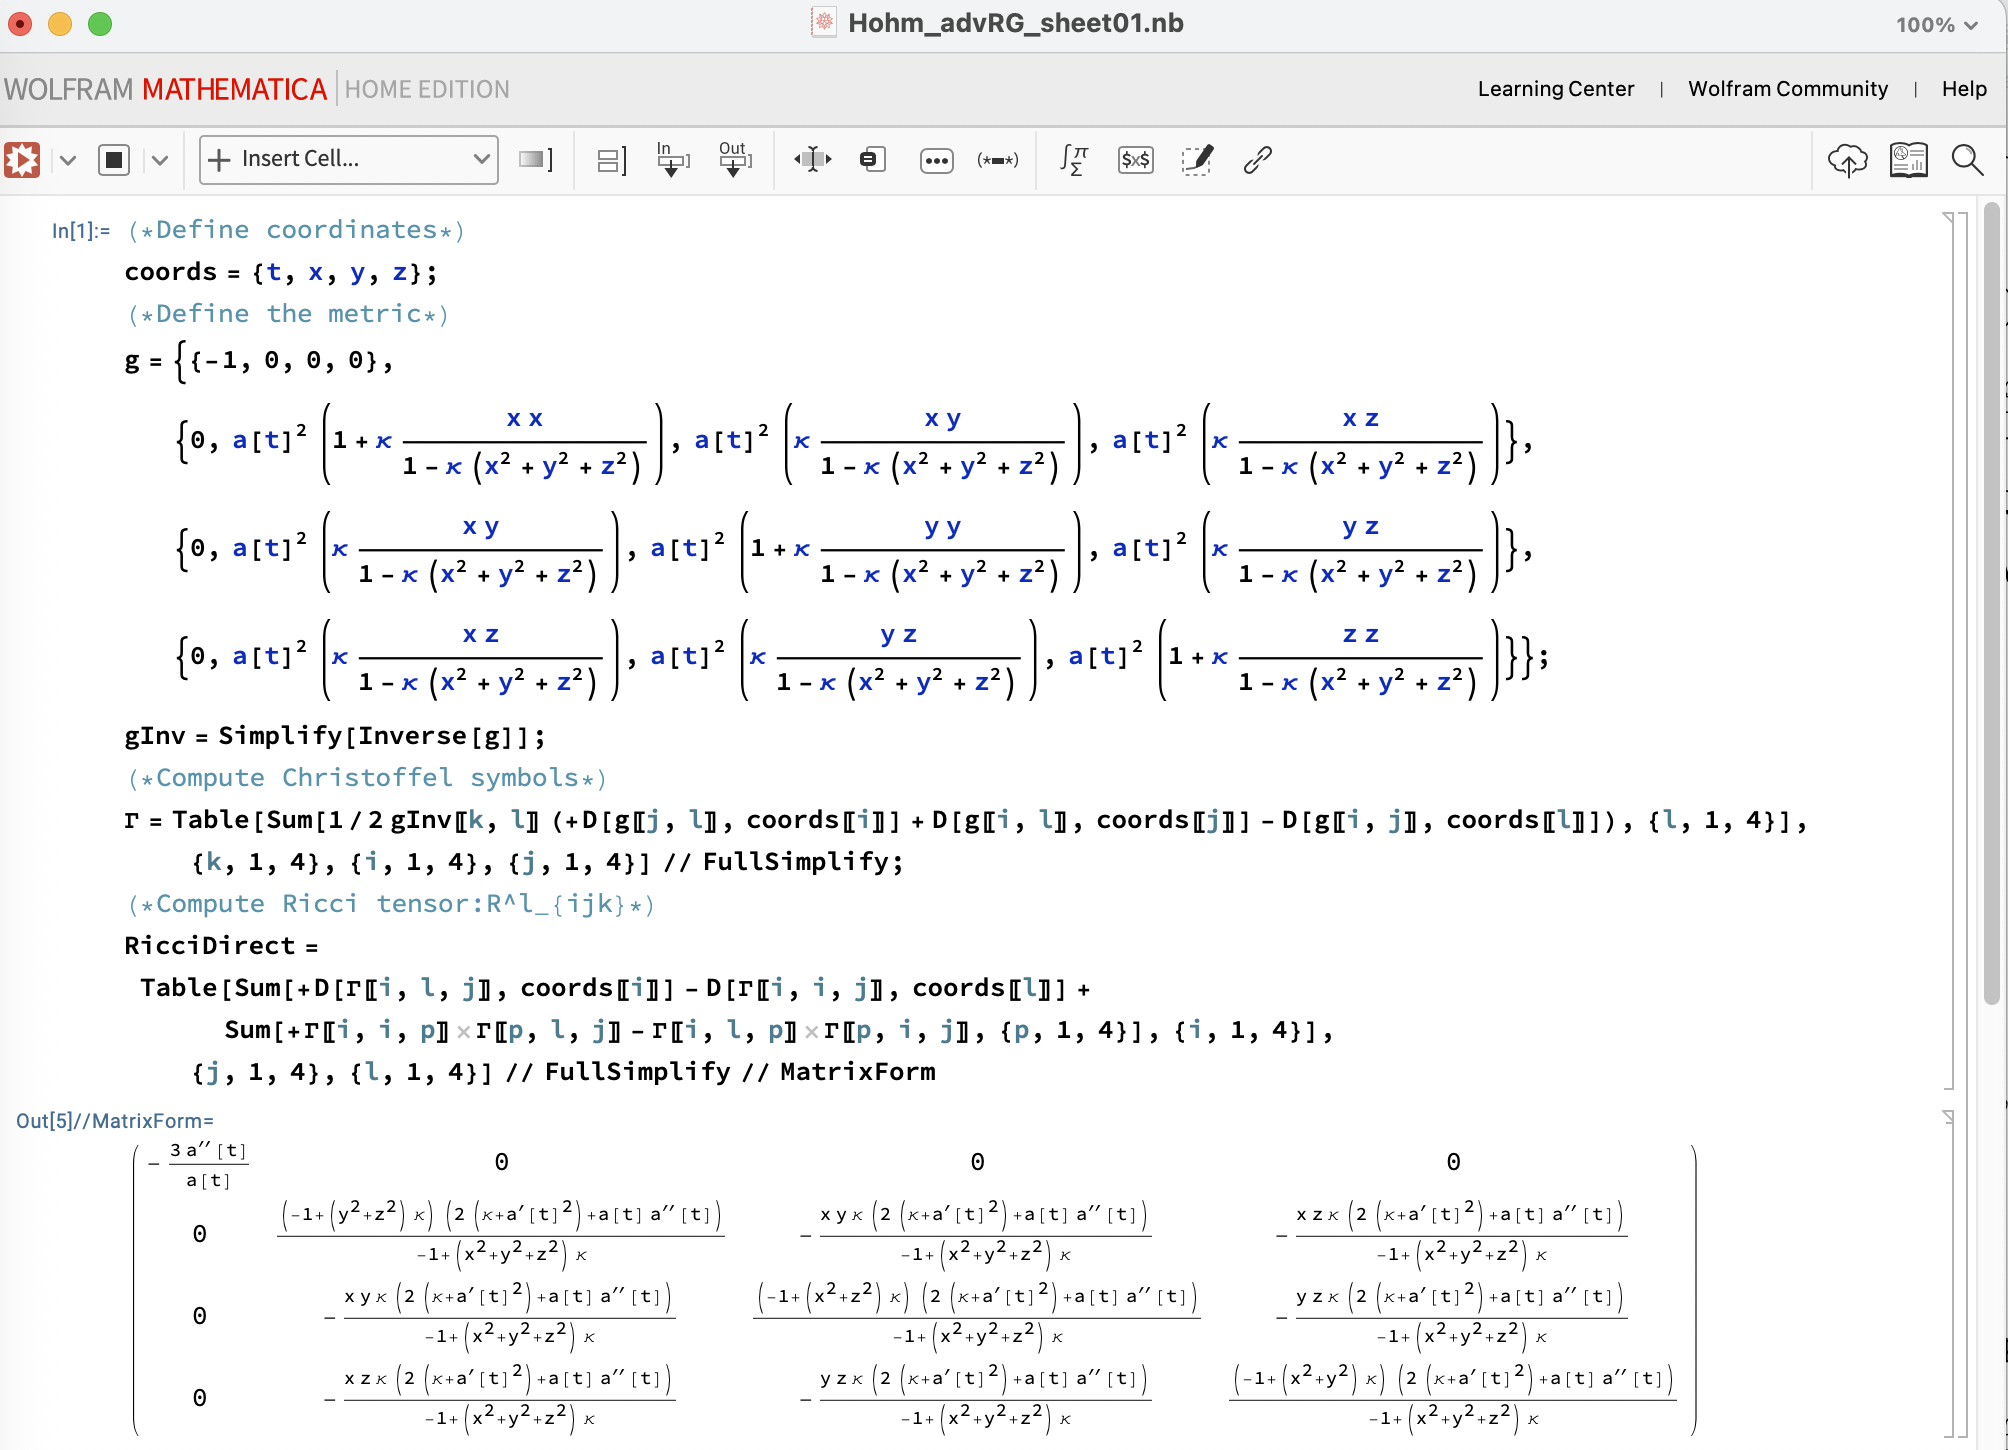
\includegraphics[width=0.95\textwidth]{/Users/christiant/MyDocuments/TeX/Hohm_AdvGR/pic_Sheet1_1a.png}
\end{figure}

\begin{align}
R_{\mu\nu}
&=\left(
\begin{matrix}
-\frac{3\ddot{a}}{a} &0\\
0 &{(a\ddot{a}+a^2+2k)\gamma_{ij}}
\end{matrix}
\right)\\
\rightarrow R&=g^{\mu\nu}R_{\mu\nu}\\
&=\frac{1}{6}\left(\frac{\ddot{a}}{a}+\frac{\dot{a}^2}{a^2}+\frac{k}{a^2}\right)
=\frac{1}{6}\left(H^2+\frac{\ddot{a}}{a}+\frac{k}{a^2}\right)
\end{align}

\item Using the Ricci tensor and the curvature scalar (from above) to build the Einstein equations. Then another Mathematica calculation gives
\begin{figure}[!h]
\centering
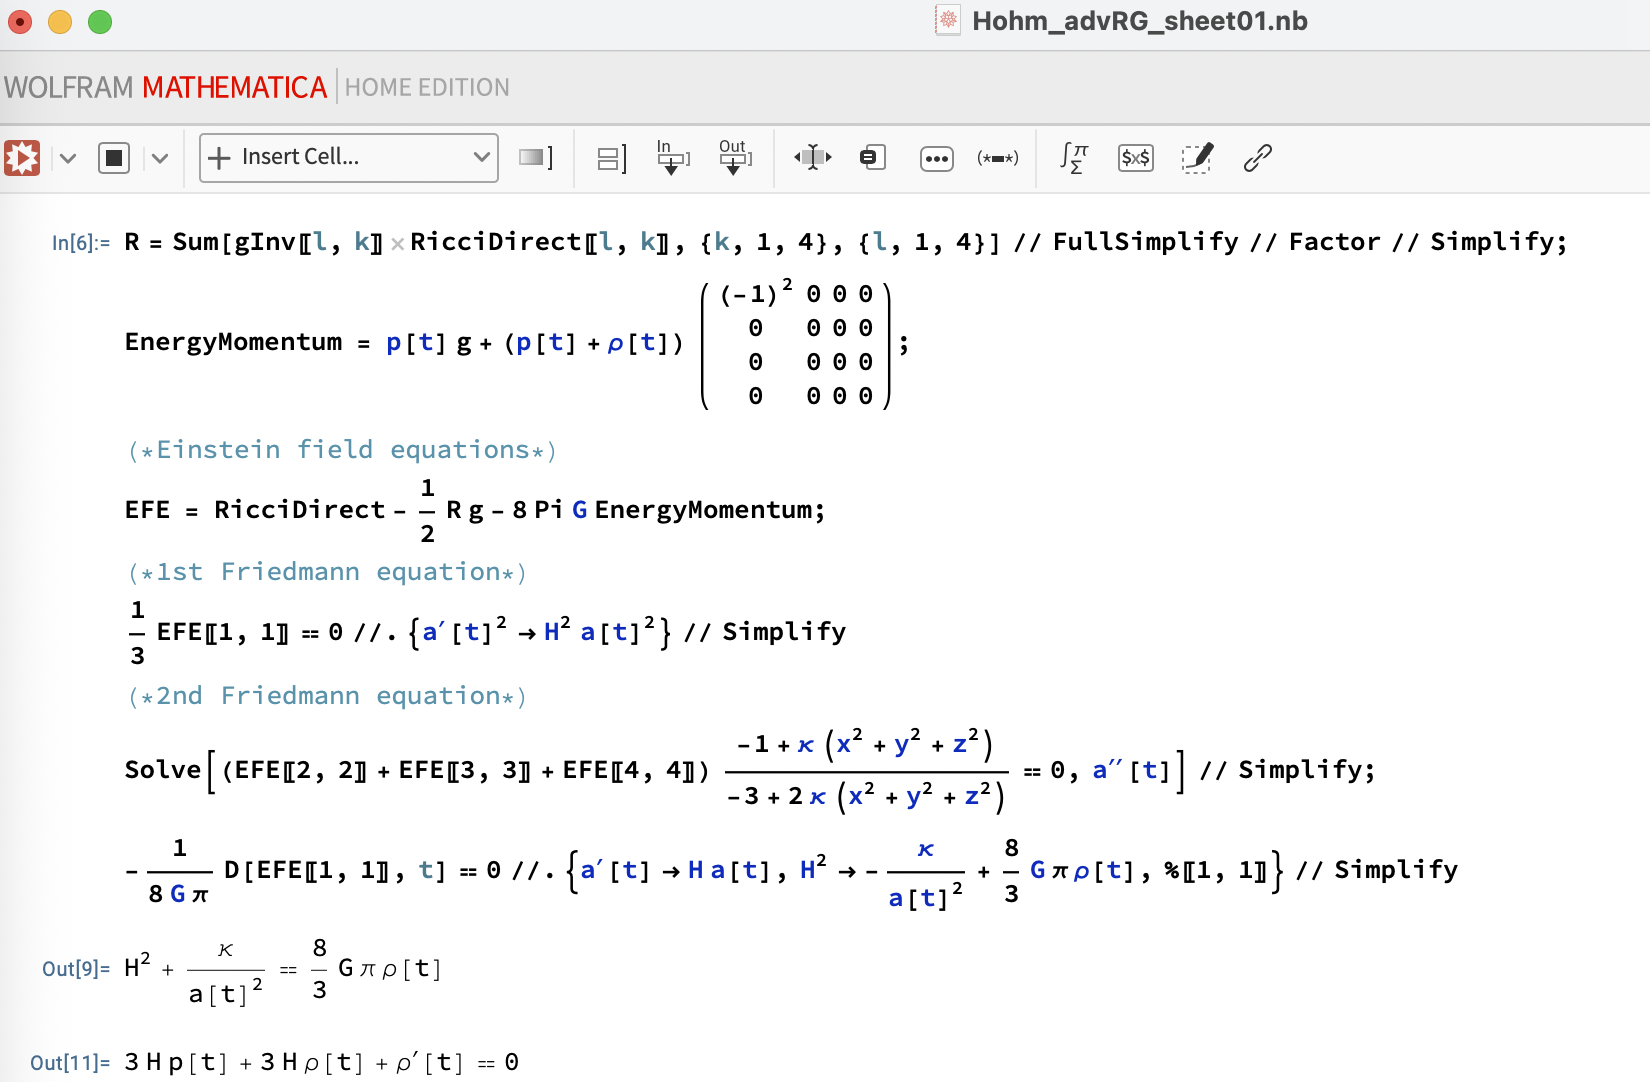
\includegraphics[width=0.95\textwidth]{/Users/christiant/MyDocuments/TeX/Hohm_AdvGR/pic_Sheet1_1b.png}
\end{figure}
\end{enumerate}

\subsection{Exercise 2 - Symmetries of the FRW metric}
\begin{enumerate}[1.]
\item With the transformation $x^i\rightarrow x'^i=x^i+K^i(x)$ we can write the Taylor expansion of the 3-metric
\begin{align}
\gamma_{ij}(x'=x+K)
&=\gamma_{ij}(x)+K^k\partial_k\gamma_{ij}(x)+\mathcal{O}(K^2).
\end{align}
Next
\begin{align}
A\equiv\frac{\partial x'^i}{\partial x^k}
&=\frac{\partial x^i+K^i(x)}{\partial x^k}\\
&=\delta^i_k+\partial_kK^i\\
\rightarrow 
A^{-1}=\frac{\partial x^k}{\partial x'^i}
&\simeq\delta^k_i-\partial_iK^k
\end{align}
because
\begin{align}
I&=A A^{-1}\\
\delta^i_j
&=\left(\frac{\partial x'^i}{\partial x^k}\right)\left(\frac{\partial x^k}{\partial x'^j}\right)\\
&=(\delta^i_k+\partial_kK^i)(\delta^k_j-\partial_jK^k)\\
&=\delta^i_j+\partial_jK^i-\partial_jK^i+\mathcal{O}(K^2)\\
&=\delta^i_j.
\end{align}
Also
\begin{align}
\gamma_{ij}(x')
&=\frac{\partial x^k}{\partial x'^i}
\frac{\partial x^l}{\partial x'^j}\gamma_{kl}(x)\\
&=\left(\delta^k_i-\partial_iK^k\right)
\left(\delta^l_j-\partial_jK^l\right)
\gamma_{kl}(x)\\
&=\gamma_{ij}(x)
-\gamma_{kj}(x)\partial_iK^k
-\gamma_{il}(x)\partial_jK^l
+\mathcal{O}(K^2)
\end{align}
and then
\begin{align}
K^k\partial_k\gamma_{ij}=-\gamma_{kj}(x)\partial_iK^k
-\gamma_{il}(x)\partial_jK^l\\
\rightarrow K^k\partial_k\gamma_{ij}+\gamma_{kj}\partial_iK^k
+\gamma_{ik}\partial_jK^k=0
\end{align}
which is equivalent to the more familiar Killing equation
\begin{align}
\mathcal{L}_K(\gamma_{ij})\equiv K_{i;j}+K_{j;i}=0
\end{align}
\item Substituting the solution into all Killing equations - proves that $K^i=a^i\sqrt{1-k|\mathbf{x}|^2}$ 
\begin{figure}[!h]
\centering
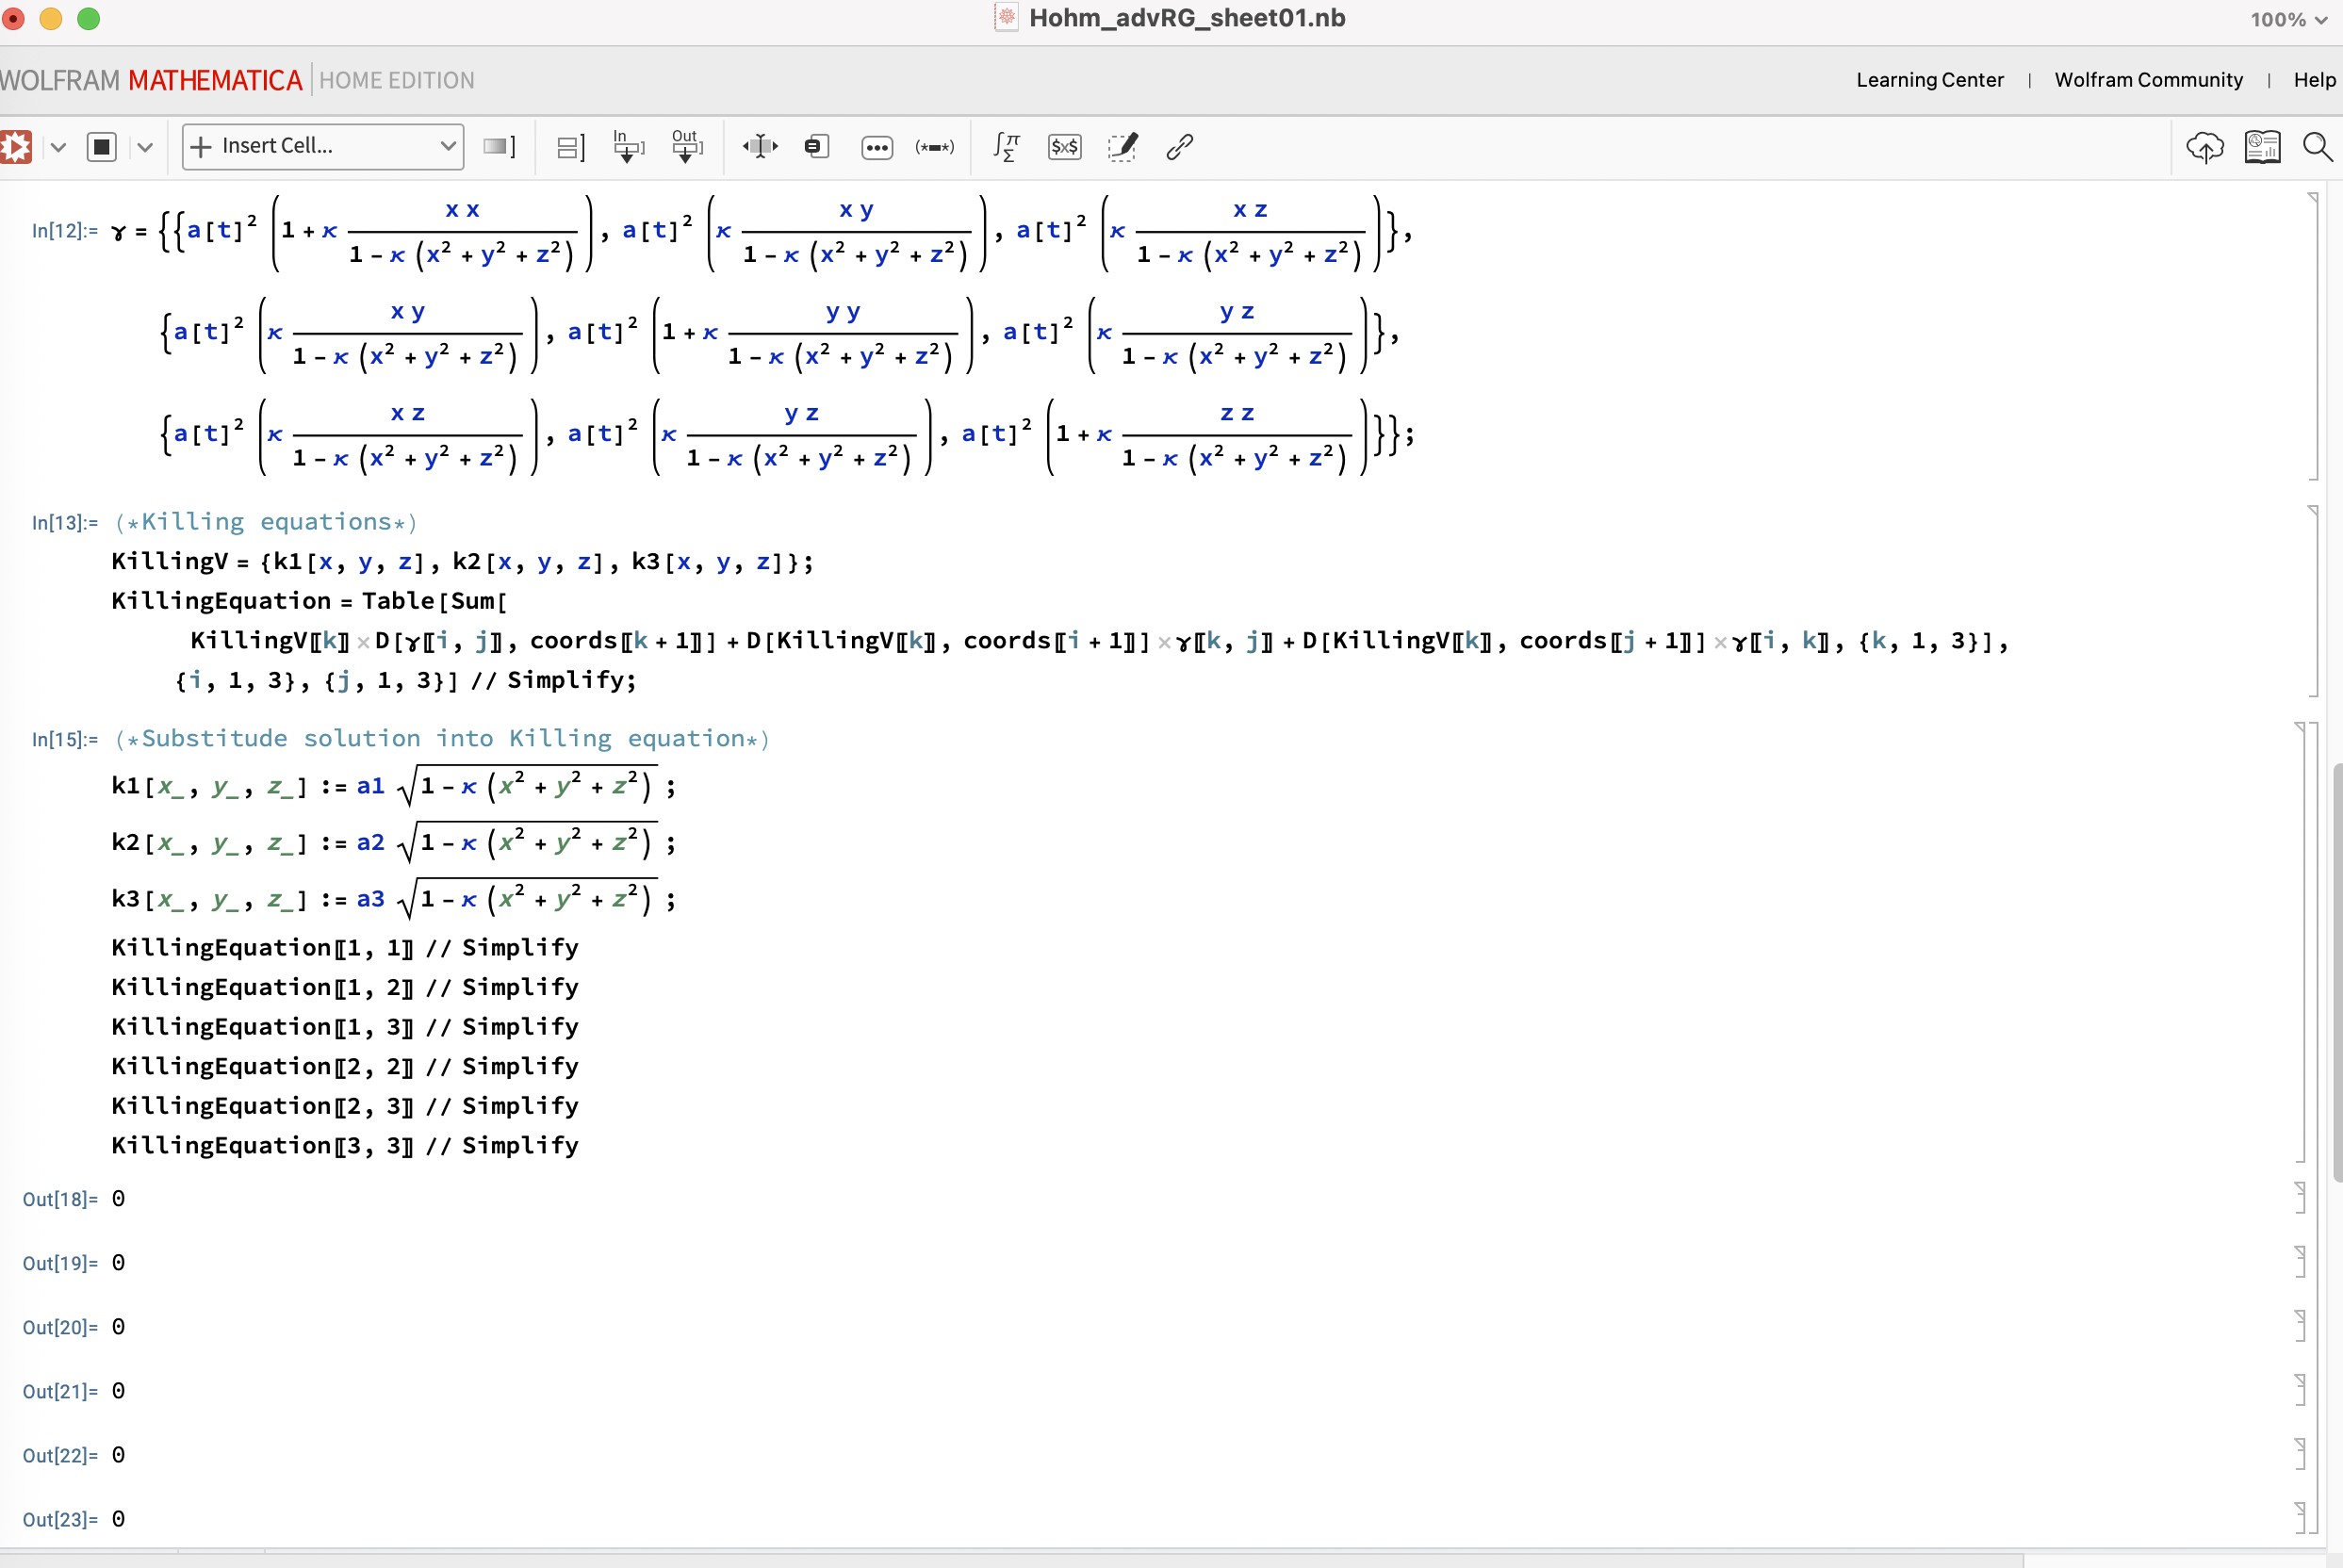
\includegraphics[width=0.95\textwidth]{/Users/christiant/MyDocuments/TeX/Hohm_AdvGR/pic_Sheet1_2b.png}
\end{figure}
\end{enumerate}


\end{document}